\chapter{觀念分子生物學}
\chapterauthor{李訓至}

\section{附錄}
\subsection{遺傳密碼表}

\begin{figure}[H]
\centering
\graphicspath{{biology/}}
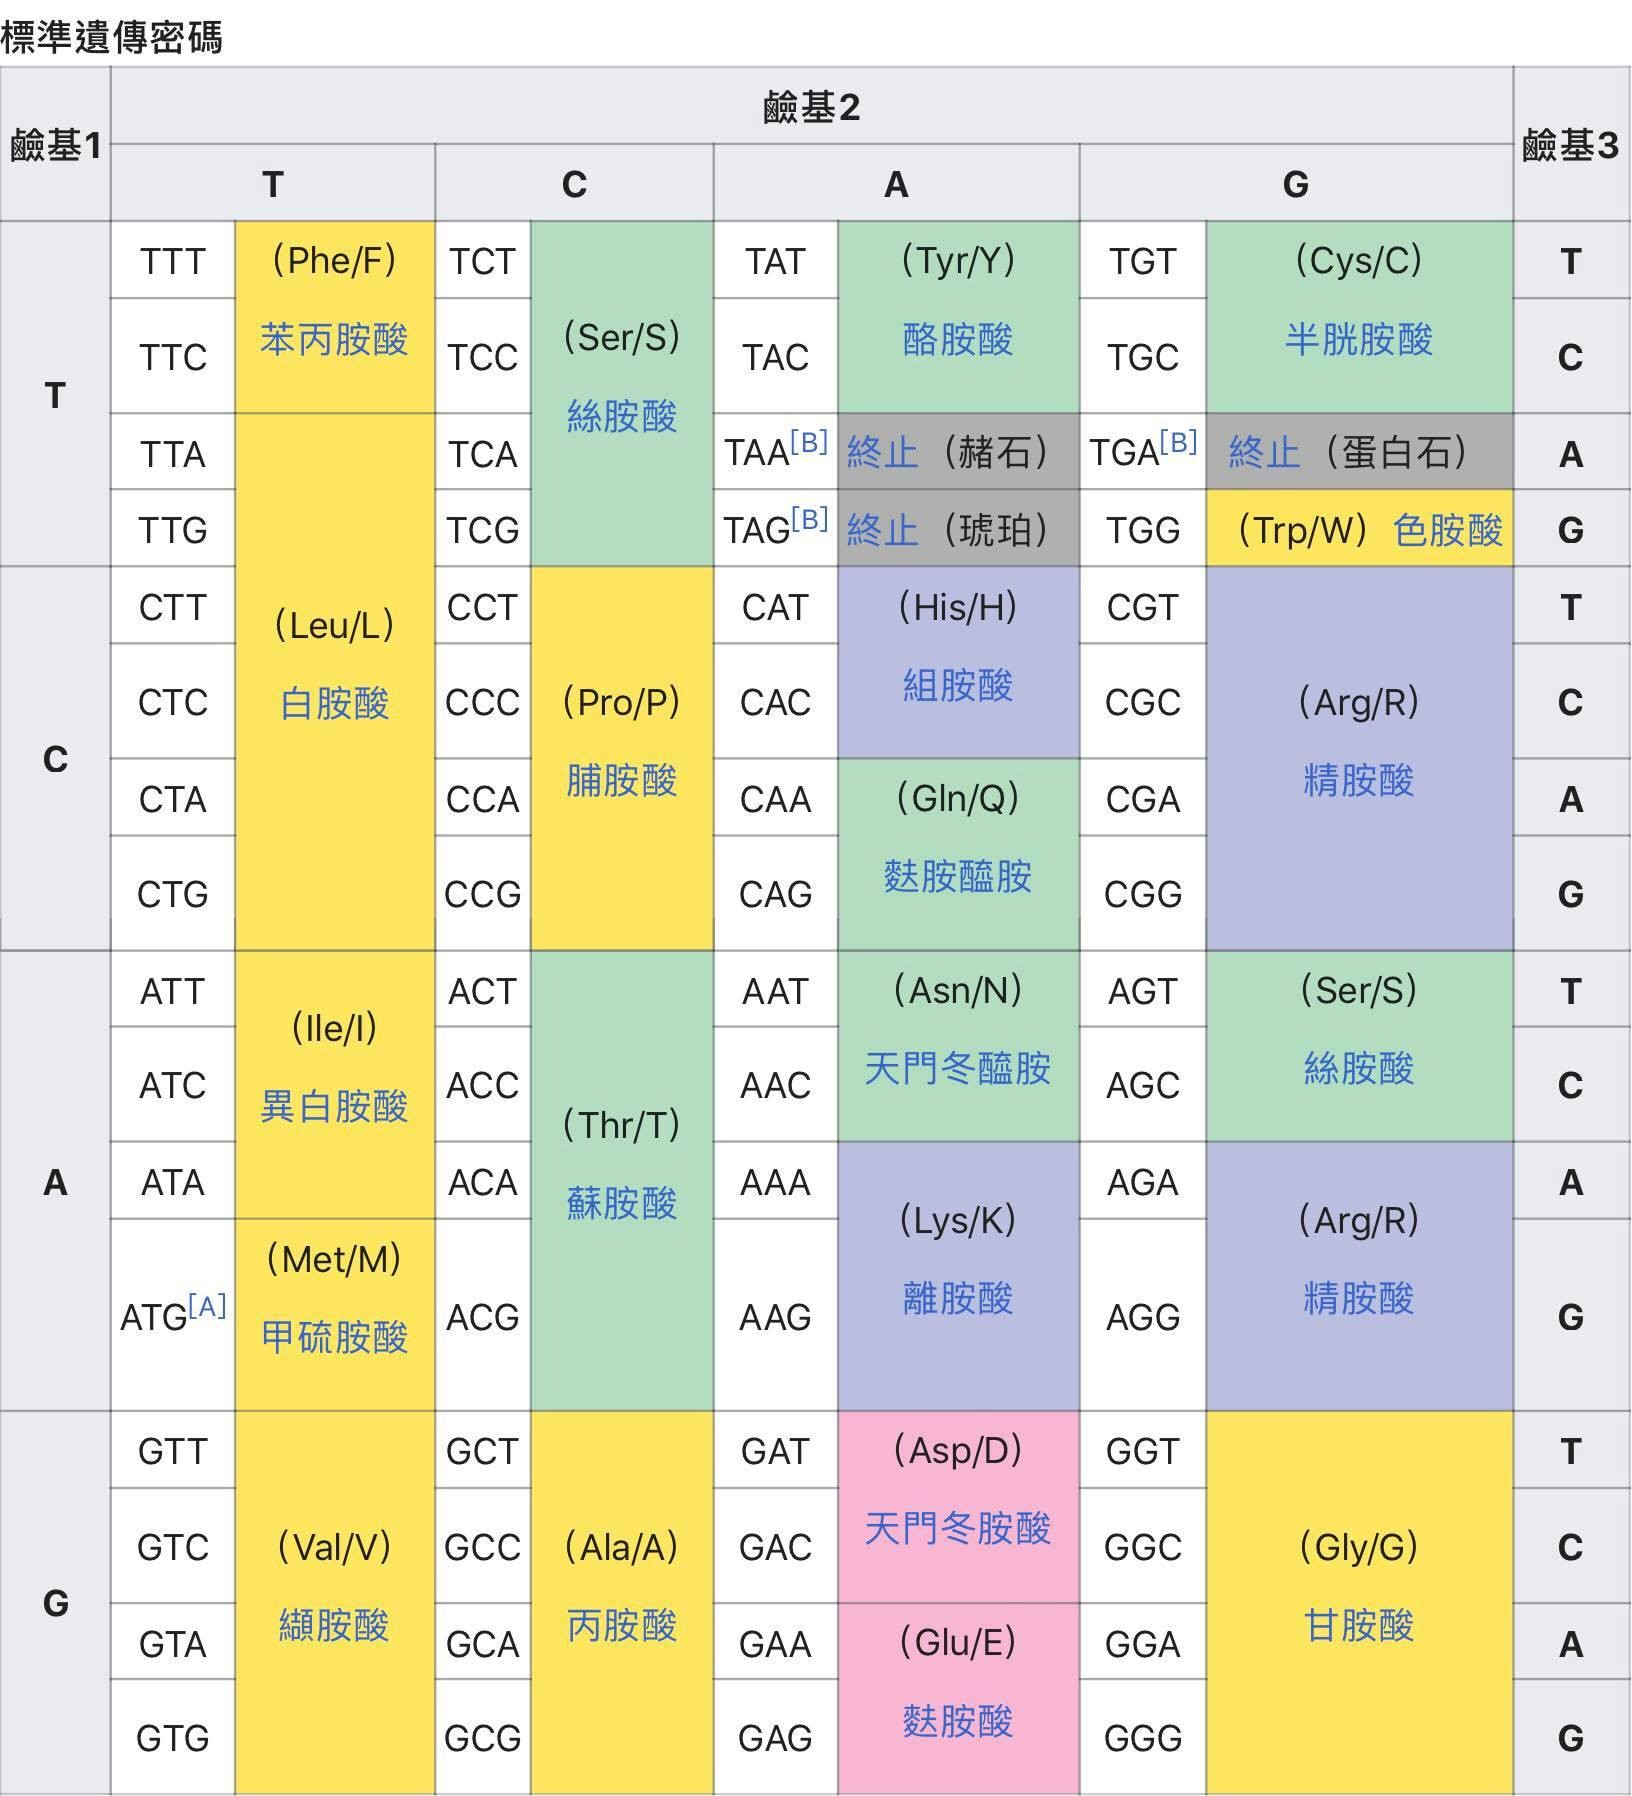
\includegraphics[width=7.5cm, center]{protein.jpg}
\caption{遺傳密碼表(from Wikipedia)} \vskip 10 pt
\label{fig:code}
\end{figure}

\subsection{分子生物學的中心教條}

\begin{figure}[H]
\centering
\graphicspath{{biology/}}
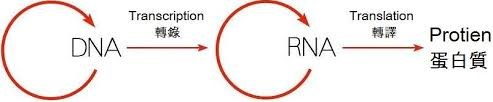
\includegraphics[width=7.5cm, center]{DNA.jpg}
\caption{分生的中心教條} \vskip 10 pt
\label{fig:DNA}
\end{figure}

\section{講師介紹}
\begin{itemize}
\item 姓名:李訓至
\item 性別:男
\item 特色:Minecraft愛好者、曾因為在英文課時沒有將英文課本拿出而多次被英文老師念、繪畫功力一流、會阻止大家刷存在
\item 名言:XXX不要刷存在
\end{itemize}